\documentclass[11pt]{article}
\usepackage[utf8]{inputenc}
\usepackage[T1]{fontenc}
\usepackage[spanish,es-noshorthands]{babel}
\usepackage[margin=2.5cm]{geometry}
\usepackage{amsmath,amssymb}
\usepackage{graphicx}
\usepackage{booktabs}
\usepackage{xcolor}
\usepackage[colorlinks=true,linkcolor=blue,citecolor=blue]{hyperref}
\usepackage{caption}
\usepackage{parskip}
\usepackage[expansion=false]{microtype}
\sloppy

\title{\textbf{La ecuación de $\beta$ óptimo, revisada con 18 curvas\\
(antes eran 6)}}
\author{Walter Quiñonez}
\date{Reporte generado con Claude Code \textperiodcentered\ 6 de septiembre de 2026}

\begin{document}
\maketitle

\begin{quote}\itshape
Este reporte repite el método de
\texttt{reporte\_formula\_beta\_optimo\_propuesta.md} (v1) con la data
nueva: ya no son 6 curvas (2 INL nominal $\times$ 3 pulsos), son 18 curvas
(6 INL nominal $\times$ 3 pulsos), con INL nominal cubriendo casi 4.4
órdenes de magnitud (2e-1 .. 4.82e-6) en vez de solo 2 valores. Además
responde la pregunta que motivó este reporte: ¿las curvas de accuracy vs
beta se aplanan a medida que el INL se achica, porque la curva P/D se
vuelve más lineal? No se modificó ningún archivo existente del proyecto ni
se corrió ningún entrenamiento nuevo.
\end{quote}

\tableofcontents

\section{La ecuación, ahora con 3$\times$ más puntos y sin el problema de confusión de v1}

v1 advertía que su exponente de $\sigma_W$ ($-3.02$) estaba determinado
por un solo contraste entre 2 grupos de INL, no por una curva de potencia
muestreada en muchos puntos. Con 6 valores de INL nominal en vez de 2, esa
objeción ya no aplica: ahora hay grados de libertad reales para poner a
prueba la forma de la ley.

\begin{table}[htbp]
\centering
\begin{tabular}{@{}lrrr@{}}
\toprule
Modelo & $R^2$ & $n$ & gl residuales \\
\midrule
solo $\sigma_W$ & 0.606 & 18 & 16 \\
solo paso medio & 0.333 & 18 & 16 \\
\textbf{combinado ($\sigma_W$ + paso medio)} & \textbf{0.938} & 18 & 15 \\
directo (INL$_{\text{real}}$ + pulsos) & 0.633 & 18 & 15 \\
\bottomrule
\end{tabular}
\end{table}

\begin{figure}[htbp]
\centering
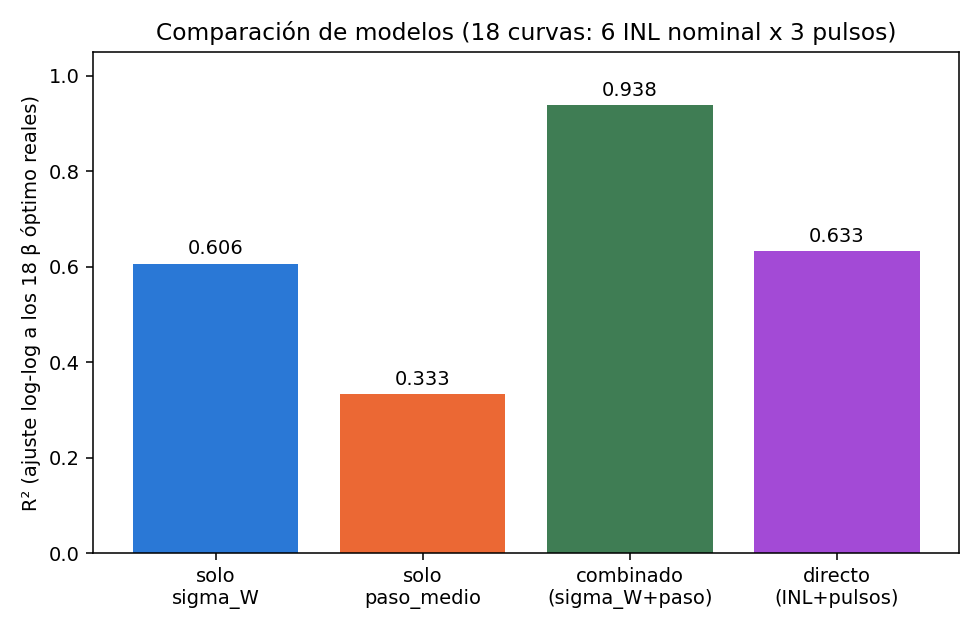
\includegraphics[width=0.75\linewidth]{comparacion_R2_v2.png}
\caption{$R^2$ del ajuste log-log de $\beta_{\text{óptimo}}$ (18 puntos reales) usando cada modelo.}
\end{figure}

La ecuación combinada:
\begin{equation}
\beta_{\text{óptimo}} \;\approx\; 1.34\times10^{-11}\cdot\sigma_W^{-3.05}\cdot\mathrm{paso\_medio}^{-0.61}
\label{eq:combinada}
\end{equation}
(exponentes: $-3.047$ para $\sigma_W$, $-0.607$ para paso medio; intercepto
$\exp(-25.05)\approx1.34\times10^{-11}$)

\textbf{Esto es la confirmación que a v1 le faltaba:} con 6 INL nominal en
vez de 2, el exponente de $\sigma_W$ sale $-3.05$, prácticamente idéntico
al $-3.02$ de v1 (ajustado con solo 2 grupos). El de paso medio sale
$-0.61$, muy cerca del $-0.64$ de v1. La ecuación combinada explica
\textbf{93.8\%} de la varianza (log-log) de los 18 $\beta$ óptimo reales,
con errores de predicción entre $-27\%$ y $+26\%$ (tabla completa en
\texttt{resultados\_formula\_propuesta\_v2.csv}).

\begin{figure}[htbp]
\centering
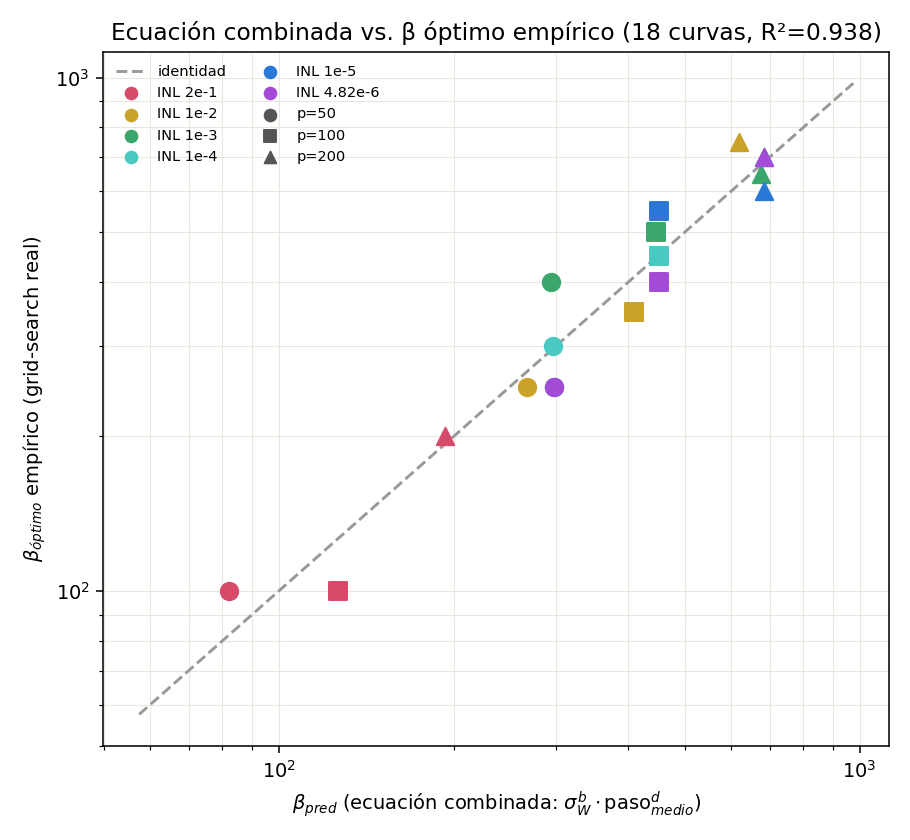
\includegraphics[width=0.7\linewidth]{beta_pred_combinada_vs_empirico_v2.png}
\caption{Ecuación combinada (\ref{eq:combinada}) vs.\ $\beta$ óptimo empírico, 18 curvas, escala log-log.}
\end{figure}

También se probó un modelo más simple y barato (sin Monte Carlo):
$\beta_{\text{óptimo}}\sim \mathrm{INL}_{\text{real}}^{b}\cdot\mathrm{pulsos}^{d}$.
Da $R^2=0.633$ --- mejor que $\sigma_W$ sola pero bastante peor que la
combinada. Confirma que $\sigma_W$ (la distribución de pesos real, vía
\texttt{G0\_initialization}) captura algo que el INL nominal por sí solo
no captura del todo.

\textbf{Limitación que sigue en pie:} $N=784$ y el dataset (MNIST) siguen
fijos en las 18 curvas, así que esos exponentes no son identificables con
esta data (absorbidos en la constante). Y aunque ahora hay 6 valores de
INL, los 4 nuevos (1e-3, 1e-4, 1e-5, 4.82e-6) están muy cerca entre sí en
el régimen ``ya casi lineal'' (Sección 2) --- la verdadera diversidad
geométrica de la curva P/D sigue concentrada en el contraste 2e-1 vs.\ el
resto, igual que en v1.

\section{``La curva P/D se vuelve más lineal cuando INL se achica'': ¿válido?}

Sí, pero hay que separar dos afirmaciones distintas que se mezclan en la
pregunta original.

\subsection{Que la curva P/D se acerca a la recta cuando INL baja --- esto es la definición de INL, no un hallazgo}

\texttt{calcular\_indice\_nl()} (la función que define INL en todo el
proyecto) es literalmente $(L-d)/d$: el exceso de longitud de la curva
sobre la distancia recta, normalizado. INL$=0$ significa curva
perfectamente lineal \textbf{por construcción}. Decir ``INL chico
$\Rightarrow$ curva más lineal'' es como decir ``un termómetro que marca
$0^\circ$C está más frío que uno que marca $100^\circ$C'': cierto, pero no
es una observación empírica sobre el sistema, es releer la definición de
la métrica.

Dicho esto, vale la pena verlo graficado para calibrar cuánto cambia la
forma, porque esa magnitud sí importa para la Sección~2.2:

\begin{figure}[htbp]
\centering
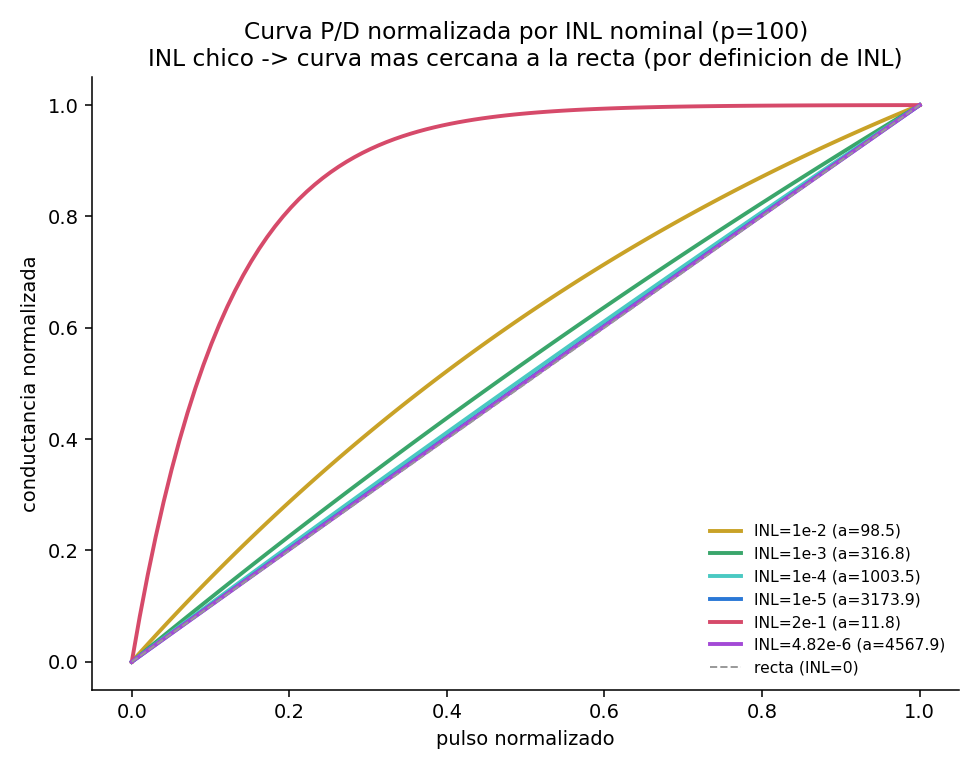
\includegraphics[width=0.75\linewidth]{curvas_PD_normalizadas_vs_INL_v2.png}
\caption{Curva P/D normalizada, una por INL nominal (p=100).}
\end{figure}

El salto grande de curvatura ocurre entre INL$=2$e-1 ($a=11.8$, muy
cóncava) e INL$=1$e-2 ($a=98.5$, moderada). De ahí para abajo (1e-3, 1e-4,
1e-5, 4.82e-6 --- cuatro órdenes de magnitud más de ``achicar el INL''),
las curvas son \textbf{visualmente indistinguibles entre sí y de la
recta} a esta escala: la curva ya ``saturó'' hacia la forma lineal mucho
antes de llegar a INL$=1$e-5. Esto es la clave para entender la
Sección~2.2.

\subsection{Que la curva de accuracy vs beta se aplana cuando INL baja --- esto SÍ es empírico, y la respuesta es ``solo parcialmente, y con matices''}

Se midieron dos descriptores de ``qué tan picuda'' es cada una de las 18
curvas accuracy-vs-beta reales:
\begin{itemize}
\item \textbf{ancho de meseta @99\%} (normalizado por $\beta_{\text{óptimo}}$):
  rango de $\beta$ alrededor del pico donde accuracy $\geq99\%$ del
  máximo, con interpolación lineal en los bordes.
\item \textbf{curvatura local en el pico}: coeficiente cuadrático de una
  parábola ajustada a los puntos cercanos al máximo (más cerca de 0 = más
  plana).
\end{itemize}

\begin{figure}[htbp]
\centering
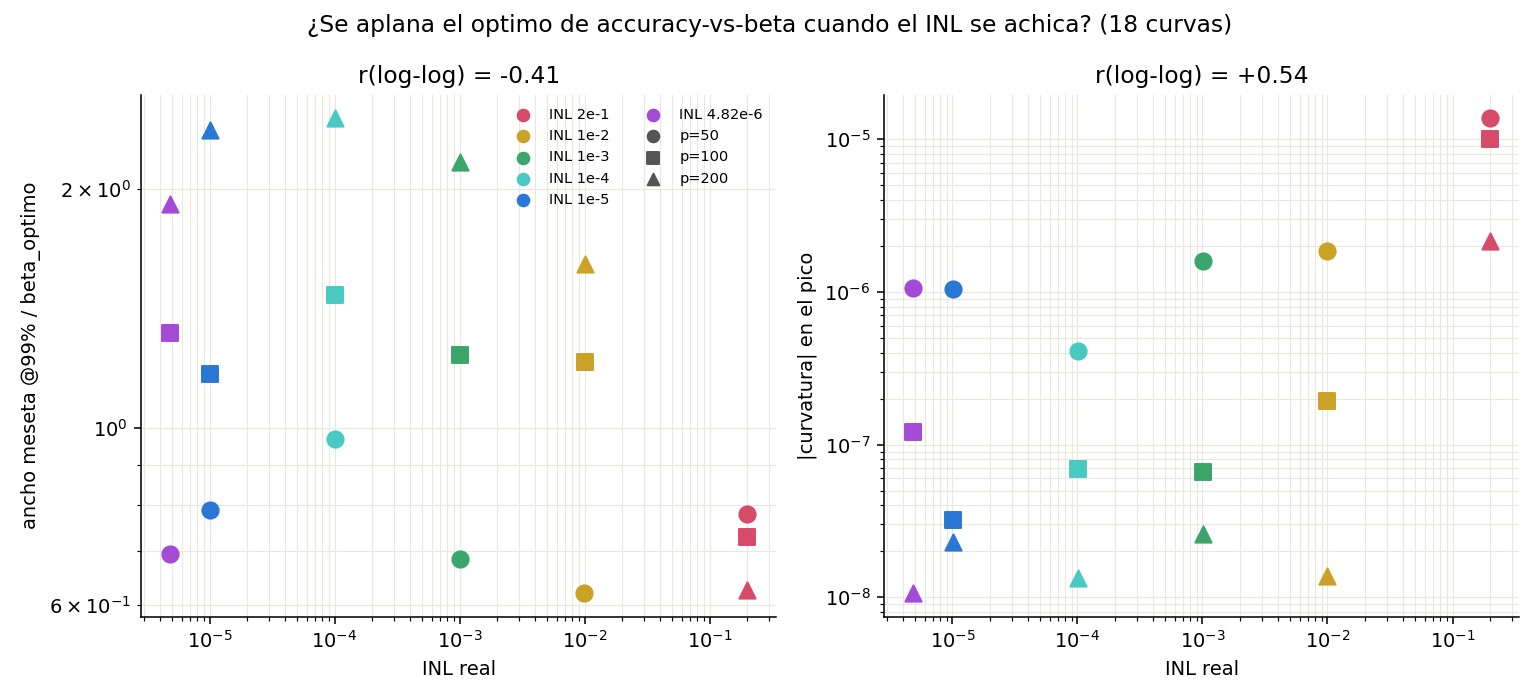
\includegraphics[width=\linewidth]{planitud_vs_INL_v2.png}
\caption{Ancho de meseta y $|$curvatura$|$ en el pico, vs.\ INL real, para las 18 curvas.}
\end{figure}

Correlación (log-log) a lo largo de las 18 curvas:

\begin{table}[htbp]
\centering
\begin{tabular}{@{}lrr@{}}
\toprule
Comparación & $r$ (18 curvas) & $r$ (15 curvas, sin INL=2e-1) \\
\midrule
INL vs.\ ancho meseta @99\%/$\beta_{\text{óptimo}}$ & $-0.41$ & $-0.12$ \\
INL vs.\ $|$curvatura$|$ en el pico & $+0.55$ & $+0.12$ \\
\bottomrule
\end{tabular}
\end{table}

\textbf{Conclusión honesta:} la correlación completa ($r=0.41$--$0.55$)
sugiere que sí, en general, INL más chico $\Rightarrow$ curva más plana.
Pero al sacar el único grupo con INL grande (2e-1) de la comparación, la
correlación \textbf{se cae a casi cero} ($r=0.12$) entre los 5 grupos
restantes (1e-2 hasta 4.82e-6, que ya cubren 4 órdenes de magnitud). Es
decir: \textbf{el ``aplanamiento'' no es una tendencia continua que sigue
creciendo a medida que INL se achica más y más} --- es, otra vez, un
efecto de \textbf{un solo contraste} (INL muy alto $=2$e-1, curva P/D muy
cóncava, óptimo de $\beta$ muy picudo) \textbf{vs.\ todo lo demás} (INL
moderado a chico, curva P/D ya casi lineal, óptimo de $\beta$ con meseta
ancha). Una vez que la curva P/D ya está ``casi lineal'' (que pasa a
partir de INL$\approx1$e-2 en este sistema, Sección~2.1), seguir bajando
el INL no aplana más el óptimo de accuracy --- coincide exactamente con
que la propia curva P/D tampoco se pone visiblemente ``más recta'' a
partir de ahí.

Esto es coherente con lo que ya había encontrado v1 sobre $\sigma_W$: con
INL nominal solo en 2 valores, cualquier tendencia ``entre grupos'' corre
el riesgo de ser, en realidad, un efecto de un único contraste. Con 6
valores de INL ahora se puede ver eso explícitamente en vez de solo
sospecharlo.

\section{Conclusión}

\begin{enumerate}
\item \textbf{La ecuación combinada de v1 se sostiene} con datos 3$\times$
  más ricos y sin el problema de confusión que v1 mismo señalaba:
  Ec.~\ref{eq:combinada}, $R^2=0.938$ sobre 18 curvas reales (antes:
  $R^2=0.947$ sobre 6, con solo 2 valores de INL). Los exponentes casi no
  se movieron ($-3.05$ vs.\ $-3.02$; $-0.61$ vs.\ $-0.64$) --- buena señal
  de que no era un ajuste espurio de v1.
\item \textbf{``INL chico $\Rightarrow$ curva P/D más lineal''} es
  verdadero por definición de INL, no un hallazgo --- pero graficarlo
  muestra que, en este sistema, la curva ya está casi saturada hacia la
  recta a partir de INL$\approx1$e-2; seguir bajando el INL otras 3-4
  décadas cambia poco su forma visible.
\item \textbf{``La curva de accuracy se aplana cuando INL se achica''} es
  cierta solo como contraste entre el régimen muy no-lineal (INL$\sim0.2$)
  y todo lo demás --- no como una tendencia continua dentro del régimen ya
  casi lineal (INL$\leq1$e-2). Los nuevos datos de INL=5e-2..5e-5
  (corriendo en el cluster al momento de este reporte) van a ayudar a
  rellenar justo la zona de transición (entre 2e-1 y 1e-2) donde,
  según este análisis, está ocurriendo casi todo el efecto --- y a
  confirmar si por debajo de 1e-2 el aplanamiento sigue plano (como
  sugieren estos 18 puntos) o si con más resolución aparece algo de
  tendencia que acá no se alcanza a ver.
\end{enumerate}

\section{Registro de códigos usados}

\begin{itemize}
\item \textbf{\texttt{estimar\_beta\_optimo\_propuesta\_v2.py}} --- Único
  script nuevo. Repite el Monte Carlo de v1 sobre las 18 curvas, agrega el
  análisis de planitud (ancho @99\% y curvatura), y las 4 regresiones
  log-log.
\item \texttt{estimar\_beta\_optimo\_propuesta.py} (v1) --- método
  original ($\sigma_W$, paso medio, Monte Carlo de corriente corregido);
  no modificado.
\item \texttt{MemCrossbarClass\_beta\_por\_capa.py}
  $\to$ \texttt{generar\_curvas\_pot\_dep()}, \texttt{G0\_initialization()}
  --- usadas sin modificar, tal como en la red real.
\item \texttt{data\_beta\_grid\_search\_SP/plot\_accuracy\_vs\_beta\_por\_INL.py}
  $\to$ \texttt{cargar\_curva()} --- reutilizada sin modificar para obtener
  la curva completa (beta, accuracy) de cada carpeta y medir su planitud.
\item \texttt{data\_beta\_grid\_search\_SP/beta\_grid\_search\_SP\_INL\_*/config\_*.json}
  --- parámetros reales de cada una de las 18 curvas P/D.
\item \texttt{data\_beta\_grid\_search\_SP/resumen\_por\_INL/resumen\_optimos.csv}
  --- los 18 $\beta$ óptimo empíricos usados para el ajuste.
\item \texttt{X\_train\_mnist.npy} --- píxeles reales muestreados
  (respetando frecuencia) en el Monte Carlo de corriente.
\end{itemize}

Archivos generados por este reporte (todos en
\texttt{formula\_beta\_optimo\_propuesta/}):
\texttt{estimar\_beta\_optimo\_propuesta\_v2.py},
\texttt{resultados\_formula\_propuesta\_v2.csv},
\texttt{coeficientes\_regresion\_v2.csv},
\texttt{curvas\_PD\_normalizadas\_vs\_INL\_v2.png},
\texttt{planitud\_vs\_INL\_v2.png},
\texttt{beta\_pred\_combinada\_vs\_empirico\_v2.png},
\texttt{comparacion\_R2\_v2.png},
\texttt{reporte\_formula\_beta\_optimo\_propuesta\_v2.tex} y este PDF.

\end{document}
